%!TEX root = ../../main.tex
\chapter{Material und Methoden}
\section{Datensatz: \ac{BraTS}}
\label{sec:Datensatz}
Der \ac{BraTS} Datensatz ist ein öffentlich zugänglicher Datensatz, der für die Entwicklung und Evaluierung von \glspl{Modell} für die Segmentierung von Hirntumoren verwendet wird. Er wurde von der Radiological Society of North America in Zusammenarbeit mit der American Society of Neuroradiology(ASNR) und Medical Image Computing and Computer Assisted Interventions(MICCAI) erstellt und besteht aus über tausend \ac{MRT} Bildern verschiedener Patienten mit Hirntumoren. \cite[vgl.][]{RSNABrainTumor2021}

\subsection{Beschreibung}
\label{subsec:Beschreibung}
Der Datensatz enthält multiinstitutionelle und multiparametrische \ac{MRT}-Scans (mpMRT), die unter klinischen Standardbedingungen mit unterschiedlichen Geräten und Protokollen aufgenommen wurden. ``Multiinstitutionell'' bedeutet, dass die Daten für den Datensatz von mehreren medizinischen Einrichtungen geliefert und zusammengeführt wurden. ``Multi-parametrisch'' bedeutet, dass der Datensatz mehrere Parameter oder Merkmale enthält, die zur Segmentierung von Hirntumoren verwendet werden können. \\
Für die Segmentierungsaufgabe wurden alle Hirntumore mit den führenden BraTS-Algorithmen segmentiert und anschließend von freiwilligen Neuroradiologie-Experten mit unterschiedlicher Erfahrung weiter verfeinert. Die manuelle Beschriftung der Daten erfolgte nach einem strengen Protokoll, um konsistente Daten zu erhalten. Abschließend wurden die manuell verfeinerten Bilder von zertifizierten und erfahrenen Neuroradiologen mit mehr als 15 Jahren Erfahrung in dieser Tätigkeit validiert. 
Die gelabelten Tumorregionen basieren auf den VASARI-Merkmalen\footnote{VASARI-Merkmale(Visually Accessible Rembrandt Images) sind ein System zur konsistenten Beschreibung von Gliomen (Tumoren) anhand definierter visueller Merkmale \cite[vgl.][]{Nam2021}}, die für einen geschulten Radiologen sichtbar sind. Zu diesen Merkmalen gehören der Gadolinium-anreichernde Tumor (Kennzeichnung 4), das peritumorale ödematöse/invasive Gewebe (Kennzeichnung 2) und der nekrotische Tumorkern (Kennzeichnung 1). \cite[vgl.][]{Baid2021}
\begin{figure}[ht]
	\centering
	\begin{subfigure}[b]{0.4\textwidth}
		\centering
		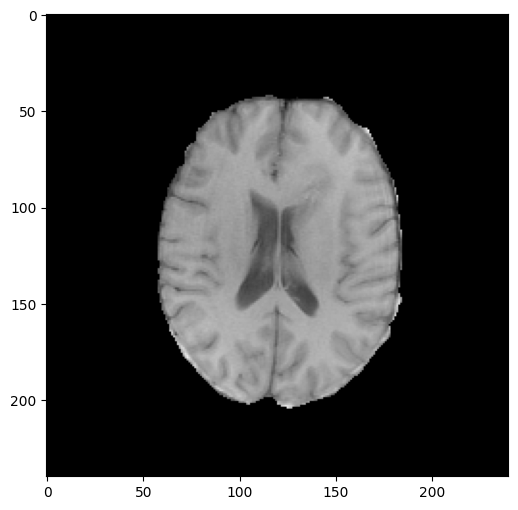
\includegraphics[width=\linewidth]{mrt_t1.png}
		\caption{T1-Gewichtung}
		\label{fig:t1}
	\end{subfigure}
	\hfill
	\begin{subfigure}[b]{0.4\textwidth}
		\centering
		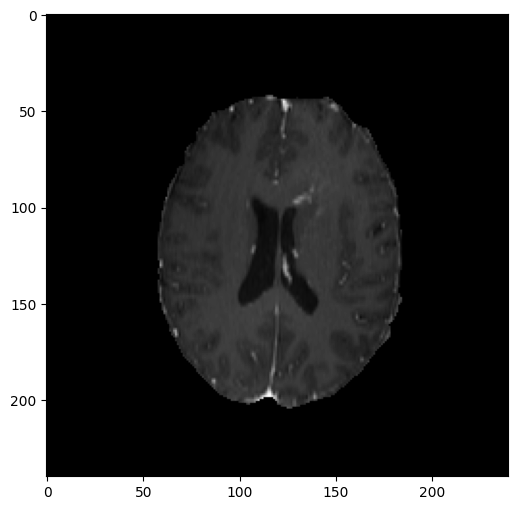
\includegraphics[width=\linewidth]{mrt_t1ce.png}
		\caption{kontrastverstärkte T1-Gewichtung}
		\label{fig:t1ce}
	\end{subfigure}
	\vskip\baselineskip
	\begin{subfigure}[b]{0.4\textwidth}
		\centering
		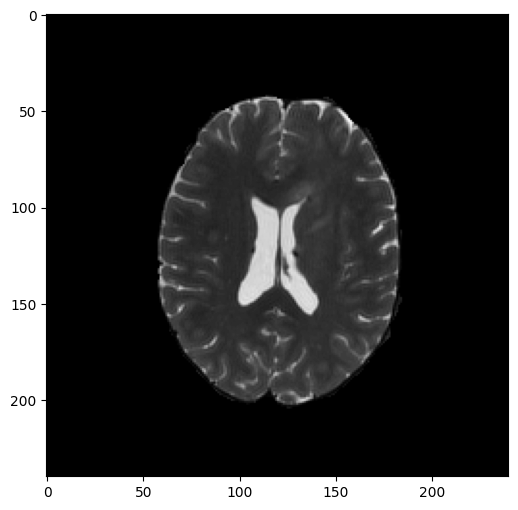
\includegraphics[width=\linewidth]{mrt_t2.png}
		\caption{T2-Gewichtung}
		\label{fig:t2}
	\end{subfigure}
	\hfill
	\begin{subfigure}[b]{0.4\textwidth}
		\centering
		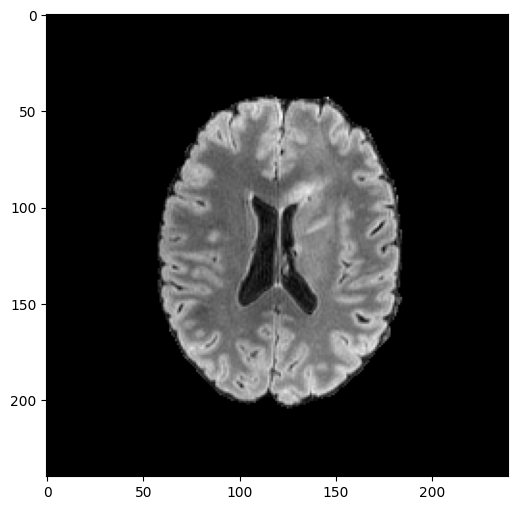
\includegraphics[width=\linewidth]{mrt_flair.png}
		\caption{Flair-Gewichtung}
		\label{fig:flair}
	\end{subfigure}
	\caption{Die vier Modalitäten des \ac{MRT} Scan im Datensatz (Quelle: Eigene Darstellung)}
	\label{fig:mrt_scans}
\end{figure} 

Der Datensatz besteht aus 1251 Einträgen, wobei jeder Eintrag aus T1, kontrastverstärkter T1, T2 und Flair Gewichtung (siehe Abb. \ref{fig:mrt_scans}) sowie einer endgültigen Segmentierung des Hirntumors besteht. Die Dateien selbst sind im NIfTI-Dateiformat, was für ''Neuroimaging Informatics Technology Initiative'' steht und ein gängiges Format für medizinische Bilddaten ist. Das Dateiformat enthält die 3D-Volumendaten, die aus mehreren Bildebenen bestehen. Jedes Voxel, ein 3D-Bildpunkt, enthält einen numerischen Wert, der das Signal oder den Kontrast wiedergibt. Zusätzlich enthält das NIfTI-Dateiformat Metadaten wie räumliche Orientierung, Bildgröße, Raumkoordinaten und weitere Metadaten. \cite[][]{NIfTI} Die Bilder liegen in einer Größe von $150\times240\times240$ Pixeln vor, was, wie bereits erwähnt, den 3D-Volumendaten entspricht, die in 150 Schichten aufgeteilt sind, wobei jede Schicht einem Bild von  $240\times240$ Pixeln entspricht.

\subsection{Vorverarbeitung}
\label{subsec:Vorverarbeitung}
Die Vorverarbeitung der Daten ist ein wichtiger Schritt, um die Qualität und Effizienz des Trainings eines neuronalen Netzes zu verbessern. Der zur Verfügung gestellte Datensatz wurde bereits einer standardmäßigen Vorverarbeitung unterzogen. Zunächst wurden die Daten vom DICOM-Dateiformat in das NIfTI-Dateiformat konvertiert, was zur einfacheren Handhabung der Daten dient. Außerdem wurde eine Anpassung an das gleiche anatomische Modell und die isotrope Auflösung vorgenommen. Abschließend wurde das Skull-Stripping durchgeführt\footnote{Skull-Stripping ist der Prozess des Entfernens des Schädels und anderer nicht-hirnbezogener Strukturen aus dem Bild. \cite[vgl.][]{SwiebockaWiek2016}} durchgeführt, um irrelevante Strukturen zu entfernen. \cite[vgl.][]{Baid2021}

\paragraph{Normalisierung}
Nach diesen Schritten sind die Daten noch nicht für das Training eines neuronalen Netzes geeignet. Die Daten müssen zunächst normalisiert werden, was auf zwei Arten geschehen kann. Entweder werden die Werte auf einen Bereich von 0 bis 1 skaliert oder es wird die Z-Normierung verwendet. Für eine einfache Skalierung der Werte wird folgende Gleichung verwendet
\begin{equation}
	f(x)=\frac{x - min(x)}{max(x) - min(x)}
\end{equation}

Dies führt zwar zu einer Vereinheitlichung der Werte, aber die Verteilung der Merkmale im Bild ist dadurch nicht normalisiert. Zu diesem Zweck wird die Z-Standardisierung verwendet, die den Mittelwert der Daten auf 0 und die Standardabweichung auf 1 setzt. Dadurch wird verhindert, dass bestimmte Merkmale gegenüber anderen dominieren. Außerdem wird die Genauigkeit des \glspl{Modell} erhöht.\cite[vgl.][]{Goodfellow2016} Die Gleichung für die Z-Standardisierung lautet
\begin{equation}
	f(x)=\frac{x - \mu_x}{\sigma_x}
\end{equation}
wobei $\mu_x$ der Mittelwert und $\sigma_x$ die Standardabweichung des Datensatzes ist. Diese Werte müssen vorab berechnet werden, in dem der Mittelwert und die Standardabweichung von jedem Bild berechnet wird, anschließend aufsummiert und durch die Anzahl der Bilder geteilt wird
\begin{equation}
	\begin{aligned}
		\mu &= \frac{1}{n}\sum_{i=1}^{n}x_i \\ \\
		\sigma &= \sqrt{\frac{1}{n}\sum_{i=1}^{n}(x_i - \mu)^2}
	\end{aligned}
\end{equation}
wobei $n$ die Anzahl der Bilder und $x_i$ ein Bild des Datensatzes ist.

\paragraph{Data Augmentation} 
Im medizinischen Bereich sind die Bilddaten oft begrenzt, was das Training eines neuronalen Netzes erschwert. Eine Methode, dem entgegenzuwirken, ist die Datenanreicherung, bei der die Vielfalt des Trainingsdatensatzes erhöht wird. Verschiedene Augmentationen sind Bildbearbeitungsmethoden wie das Drehen, Skalieren, Beschneiden oder auch Spiegeln eines Bildes. Es ist darauf zu achten, dass alle Augmentierungen sowohl auf die Eingabebilder als auch auf die zugehörigen Segmentierungen angewendet werden, da das Neuronale Netz sonst falsche Masken für die Eingaben lernt. \cite[vgl.][]{Shorten2019}

\paragraph{3D-Bild zu 2D-Bilder} 
Die Daten liegen als 3D-Bilddaten vor, jedoch ist die Datenmenge mit 1251 Bildern recht gering. Um mehr Bilder aus den vorhandenen Daten zu erhalten, werden die 3D-Bilder in einzelne 2D-Bilder geschnitten. Wie bereits im Abschnitt \ref{subsec:Beschreibung} erwähnt, besteht ein 3D-Bild aus 150 Schichten mit einer Größe von $240\times240$ Pixeln. Jede einzelne Schicht wird als separates Bild gespeichert, um die Datenmenge zu erhöhen, so dass aus einem 3D-Bild 150 einzelne 2D-Bilder entstehen. Dadurch erhöht sich nicht nur die Datenmenge, sondern auch die Berechnungsgeschwindigkeit, da in der zweidimensionalen Darstellung weniger Rechenleistung und Speicherplatz benötigt wird. Die Umwandlung von 3D- in 2D-Bilder hat aber auch Nachteile, wie den Verlust des räumlichen Zusammenhangs zwischen den einzelnen Schichten. \cite[vgl.][]{Stevens2020}

\paragraph{Größen Skalierung}
\label{paragraph:GrößenSkalierung}
Bei einigen neuronalen Netzen kann die Bildgröße eine Rolle spielen. Es gibt Architekturen, bei denen die Bildgröße beliebig sein kann oder bei denen das Eingabebild eine bestimmte Größe haben muss, um verarbeitet werden zu können. \\
Die für die Segmentierung verwendete Architektur ist ein U-Net und wird im Kapitel \ref{sec:Modellarchitektur} genauer beschrieben. Aufgrund der speziellen Architektur des U-Net müssen die Bilder eine bestimmte Größe haben. Der Grund für die spezifische Eingabegröße liegt in der Architektur des U-Net, genauer gesagt in den Down- und Upsampling-Pfaden. Durch Faltungs- und Max-Pooling-Schichten wird die Bildgröße auf der einen Seite schrittweise verkleinert und auf der anderen Seite wieder vergrößert. \\
Aufgrund des Designs des U-Net muss die Bildgröße ein Vielfaches der Anzahl der Downsampling-Layer sein. Die Größe der Bilder ist durch $2^N$ definiert, wobei $N$ die Anzahl der Downsampling-Schichten ist. Wenn $N=4$, dann muss die Eingabegröße der Bilder ein Vielfaches von $2^4=16$ sein. Wenn die Größe nicht korrekt ist, kann es zu Inkonsistenzen zwischen den Größen kommen, was wiederum die Performance des \gls{Modell}s beeinträchtigt. \cite[vgl.][]{Ronneberger2015}

Um die Bilder auf eine geeignete Größe zu bringen, werden sie von der Mitte nach außen abgeschnitten. Die Größe des Bildausschnitts beträgt grundsätzlich $128\times128$ Pixel. Es kann jedoch vorkommen, dass Teile des Gehirns abgeschnitten werden (siehe Abb. \ref{fig:GrößeOhnePuffer}), daher wurde ein Puffer von 60 Pixeln pro Rand hinzugefügt. Nach dem Hinzufügen des Puffers hat das Bild nicht mehr die passende Größe und wird schließlich auf $128\times128$ Pixel skaliert (siehe Abb. \ref{fig:GrößePuffer}).
\begin{figure}[ht]
	\centering
	\begin{subfigure}[b]{0.4\textwidth}
		\centering
		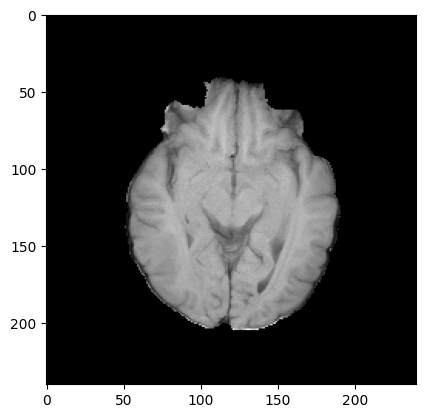
\includegraphics[width=\linewidth]{img_size_original.png}
		\caption{Original Bild}
		\label{fig:GrößeOrg}
	\end{subfigure}
\vfil
	\begin{subfigure}[b]{0.4\linewidth}
		\centering
		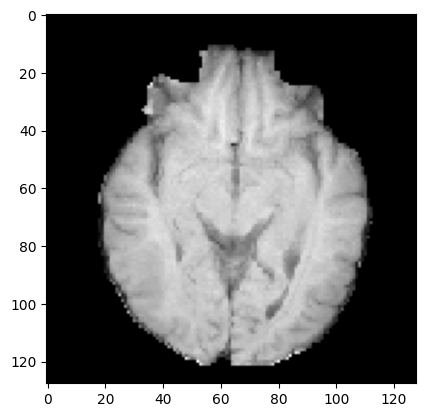
\includegraphics[width=\textwidth]{img_size_crop_puffer.png}
		\caption{Ausschnitt mit Puffer}
		\label{fig:GrößePuffer}
	\end{subfigure}
\hfil
	\begin{subfigure}[b]{0.4\linewidth}
		\centering
		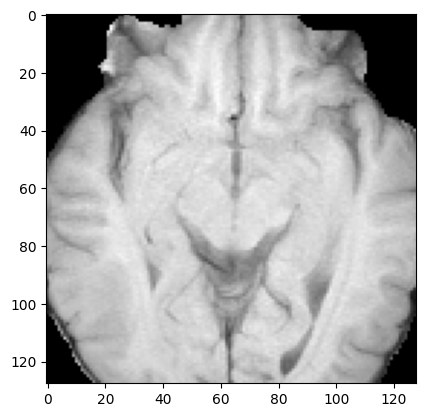
\includegraphics[width=\textwidth]{img_size_crop.png}
		\caption{Ausschnitt ohne Puffer}
		\label{fig:GrößeOhnePuffer}
	\end{subfigure}
	\caption{Orginal Bild (T1-Gewichtung) im Vergleich zum Ausschnitt mit und ohne Puffer. (Quelle: Eigene Darstellung)}
\end{figure} 


\subsection{Aufteilung}
Für eine erfolgreiche Modellentwicklung ist es wichtig, den Datensatz in verschiedene Teile aufzuteilen. Zu diesem Zweck wird der Datensatz in einen Trainingsdatensatz, einen Validierungsdatensatz und einen Testdatensatz unterteilt. Diese verschiedenen Datensätze ermöglichen es, die Leistungsfähigkeit und Generalisierbarkeit des \gls{Modell}s zu beurteilen. \\
Der Trainingsdatensatz wird verwendet, um das Modell zu trainieren, indem die internen Modellparameter anhand der Eingabedaten und der zugehörigen Labels angepasst werden. Je größer der Trainingsdatensatz ist, desto besser kann das \gls{Modell} generalisieren, da es viele Daten mit unterschiedlichen Merkmalen lernt. \\
Der Validierungsdatensatz wird verwendet, um die Leistung des \gls{Modell}s während des Trainings zu bewerten. Anhand der Ergebnisse des Validierungsdatensatzes werden die Hyperparameter des \gls{Modell}s angepasst. Es ist darauf zu achten, dass sich dieser Datensatz nicht mit dem Trainingsdatensatz überschneidet, da es sonst zu falschen Ergebnissen kommt. \cite[vgl.][]{Weidman2020} Will man das Modell abschließend noch einmal evaluieren, wird häufig ein Testdatensatz verwendet, den das \gls{Modell} noch nie gesehen hat. Nach Abschluss des Trainings kann der Testdatensatz verwendet werden, um die endgültige Leistungsfähigkeit des \glspl{Modell}s zu beurteilen. \\
Die Aufteilung der Daten sollte so gewählt werden, dass der Trainingsdatensatz genügend Daten enthält, um das neuronale Netz zu trainieren. Es ist darauf zu achten, dass ebenfalls genügend Daten für den Validierungs- und Testdatensatz verbleiben, um eine aussagekräftige Bewertung des \gls{Modell}s zu ermöglichen. Die Aufteilung wie sie hier in der Arbeit verwendet wird liegt bei $70:30$, wobei sich die $30\%$ halbieren und je $15\%$ für Validierungs- und Testdatensatz verwendet werden.